\section{PCB Specifications}

\begin{table}[h!]
\centering
\begin{tabular}{l|p{0.64\textwidth}}
\toprule
\textbf{Parameter} & \textbf{Specification} \\ \bottomrule
Substrate Material & \textcolor{orange}{\hyperref[subsec:RO3003]{Rogers RO3003}: the simulations are built on it. \hyperref[subsec:selectedPCBsubstrate]{Rogers TMM10i} is the validation substrate.} \\
Conductive Layer & Copper + Gold Plating over a non-magnetic adhesion layer\footnotemark \\
Vias & Solid copper, gold plated over a non-magnetic adhesion layer \\
Target Impedance & 50 $\Omega$ \\
Frequency Range & 9 kHz -- 18 GHz\ \footnotemark\\
% PCB design Tool & Altume \\
connector type & SMP (Amphenol RF 925-NM196J-51P non-magnetic) \\
connector count & one version with 2 ports and one with 6 ports \\
Transmission Line & Coplanar Waveguide (CPW) \\
\quad Substrate Height ($h$) & \textcolor{orange}{0.381 mm (0.015 in) in all simulations. Standard for TMM10i, but \emph{not} a standard RO3003 thickness (0.127, 0.254, 0.508, 0.762 and 1.524 mm): it has to be special-ordered, or the design changes.} \\
\quad Trace Width ($w$) & \textcolor{orange}{RO3003: 0.40 mm. TMM10i: 0.20 mm. (50 $\Omega$, the CPW model of the simulations, 35 $\mu$m copper, lid relief 0.3 mm over the line.)} \\
\quad Gap Width ($s$) & \textcolor{orange}{RO3003: 0.104 mm. TMM10i: 0.247 mm. (Same model.)} \\
Chip Mounting Cavity &\textcolor{orange}{opening $6.5\times6.5$ mm$^2$ through the board, for the $6.3\times6.3\times0.381$ mm$^3$ die (0.1 mm clearance on every side)\ \footnotemark}\\
Manufacturer & \textcolor{red}{\textbf{??}} \\
\bottomrule
\end{tabular}
\end{table}
\footnotetext[\numexpr\value{footnote}-2]{make sure that the adhesion layer is not magnetic -- check EPIG (Electroless Palladium Immersion Gold)}
\footnotetext[\numexpr\value{footnote}-1]{18GHz is the limit of the SMP connectors we have. option to buy \href{https://www.svmicrowave.com/smpm-male-non-magnetic-pcb-surface-mount-connector-fd}{up-to 20GHz connector}.}
\footnotetext[\numexpr\value{footnote}]{drilled through in the model: the die is as thick as the board (0.381 mm), so their top faces are flush. The alternative is a blind pocket.}

\begin{figure}[h]
    \centering
    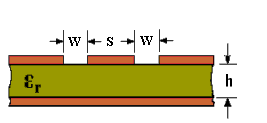
\includegraphics[width=0.5\linewidth]{tex/CPW.png}
\end{figure}
